% 10-30 páginas

\chapter{Redes Complexas} \label{cap:redes}

\begin{section}{Introdução} \label{sec:redes-complexas}

No domínio de agrupamento de software, é comum representar um sistema de software através de um grafo que modela as dependências entre entidades do software. Essa representação é conveniente porque a teoria dos grafos possui muitos teoremas e algoritmos que se aplicam a grafos. Mais recentemente, grafos têm sido objeto de estudo de um ramo da física estatística denominado teoria das redes complexas. Este capítulo descreve alguns avanços dessa teoria que são relevantes para o problema de agrupamento de software abordado neste trabalho.

A teoria das redes complexas estuda propriedades gerais de diversos tipos de redes, representadas como grafos, com o uso de ferramentas estatísticas. Estudos realizados na última década revelaram similaridades entre redes estudadas em diversos domínios. Exemplos incluem redes tecnológicas, como a Web e a rede de distribuição de energia elétrica dos Estados Unidos, redes biológicas, como cadeias alimentares e redes de ligações entre proteínas, e redes sociais, como as relações de amizade entre alunos de uma escola.

O termo ``rede'' em geral está associado a entidades reais, como pessoas e relacionamentos de amizade, enquanto o termo ``grafo'' designa uma abstração matemática conveniente para representar relacionamentos entre objetos. Na teoria das redes complexas, no entanto, os termos são frequentemente usados como sinônimos, e é desta forma que eles são usados neste trabalho.

Barabási e Albert \cite{Barabasi1999} analisaram uma amostra da \emph{World Wide Web}, modelada como um grafo não-orientado no qual os vértices representam páginas e as arestas representam \emph{links} entre duas páginas. Eles observaram a distribuição dos graus dos vértices, isto é, o número de vértices conectados a outros $k$ vértices ($N(k)$), para cada valor de $k > 0$, e encontraram uma lei de potência, isto é, acharam $N(k)$ proporcional a $k^{-\gamma}$, como mostra a Figura \ref{fig:leidepotencia}. Desde então, leis de potência têm sido encontradas na distribuição de graus de redes estudadas em diversos domínios, inclusive no domínio de software, com $\gamma$ variando tipicamente entre 2 e 3. Redes com esse padrão são chamadas de \emph{redes livres de escala}.

% Eles perceberam que o número de vértices com grau $k$, isto é, vértices ligados a outros $k$ vértices, era aproximadamente proporcional a $k^{-\gamma}$, função conhecida como lei de potência (veja a Figura \ref{fig:leidepotencia}). Desde então, esse padrão de conectividade tem sido encontrado em redes estudadas em diversos domínios, inclusive no domínio de software. Redes com esse padrão são chamadas de redes \emph{livres de escala}.

% Explicar que não há valor característico para o grau de um vértice, e daí vem o nome.

\begin{figure}[htbp]
	\centering
	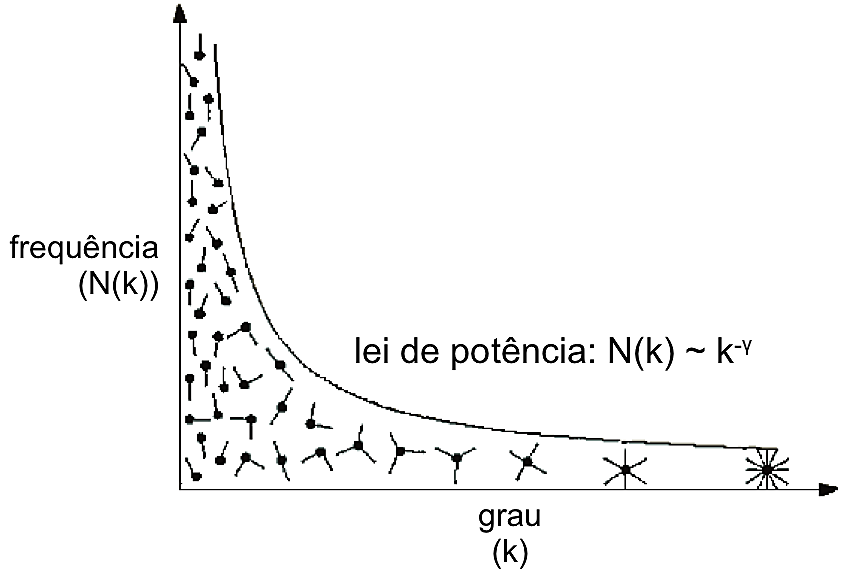
\includegraphics[width=0.6\textwidth]{figuras/leidepotencia}
	\caption{Distribuição do número de arestas por vértice do tipo lei de potência. Adaptado de \cite{Barabasi2007}.}
	\label{fig:leidepotencia}
\end{figure}

% No caso de redes orientadas, há duas distribuições a serem consideradas: a distribuição dos graus de entrada e a distribuição dos graus de saída. Nas redes orientadas que são livres de escala, ambas as distribuições seguem leis de potência.

% e alto coeficiente de agrupamento
Estudos recentes têm aplicado a teoria das redes complexas a redes de dependências estáticas entre entidades do código-fonte (funções, classes etc.) de sistemas de software. (Daqui pra frente, tais redes serão denominadas \emph{redes de software}, em contraste com redes biológicas, redes sociais etc.) Valverde e Solé \cite{Valverde2003} estudaram redes não-orientadas formadas por relações de agregação de tipos em diagramas UML, programas em C e programas em C++. Myers \cite{Myers2003} analisou redes de chamadas de função em programas em C e redes de agregação e herança em programas em C++, modeladas como grafos orientados. Em ambos os casos as redes foram identificadas como livres de escala. 

Redes livres de escala também foram encontradas em programas escritos em Smalltalk \cite{Marchesi2004,Concas2007} e em Java \cite{Hyland-Wood2006,Baxter2006,Ichii2008}, em dependências entre pacotes de software \cite{Labelle2004}, em dependências entre bibliotecas dinâmicas \cite{Louridas2008} e até mesmo em referências entre objetos em tempo de execução \cite{Potanin2005}.

Se diversas redes possuem um mesmo padrão de distribuição de graus, o que as diferencia? Milo e outros pesquisadores \cite{Milo2002} estudaram a estrutura de redes orientadas de diversos domínios em busca da resposta. Para isso, eles listaram 13 possíveis configurações de arestas em redes com 3 vértices --- as chamadas tríades ---, mostradas na Figura \ref{fig:triades}. Contando o número de vezes que cada tríade aparece em uma rede, é possível formar um vetor, denominado \emph{perfil de concentração de tríades} (PCT), que é característico de redes de um domínio. A Figura \ref{fig:tcp} mostra, lado a lado, PCTs de redes de dois domínios distintos. É notável a diferença nas concentrações das duas primeiras tríades (de cima para baixo).

\begin{figure}[htbp]
	\centering
		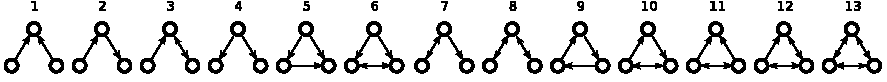
\includegraphics[scale=1]{figuras/triads}
	\caption{Tríades, ou grafos com três vértices, numeradas de 1 a 13.}
	\label{fig:triades}
\end{figure}


\begin{figure}[htbp]
	\centering
		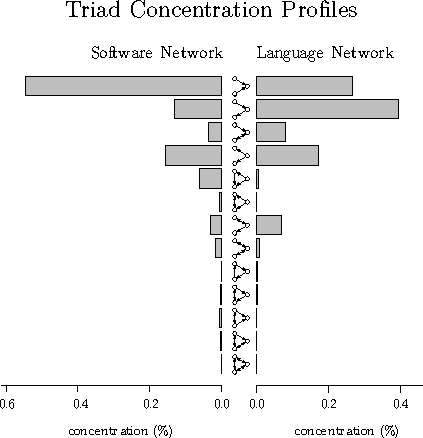
\includegraphics[scale=1]{figuras/tcp}
	\caption{Perfis de concentração de tríades de duas redes distintas. À esquerda, rede de dependências entre as classes do programa JabRef, versão 2.5b2. À direita, rede de adjacências entre palavras da língua japonesa \cite{Milo2004}.}
	\label{fig:tcp}
\end{figure}

\end{section}

\begin{section}{Modelos de Síntese de Redes Organizadas em Módulos}
% deu 7 páginas

Para tentar explicar os mecanismos responsáveis pela formação de redes livres de escala em diversos domínios, vários modelos de redes livres de escala foram propostos. Os modelos são algoritmos que geram vértices e arestas de forma probabilística porém de acordo com certas regras que garantem que, quando o número de vértices tende a infinito, a distribuição dos graus dos vértices tende a uma lei de potência. Tais modelos, portanto, geram redes similares a redes de software, ao menos quanto à distribuição dos graus.

Para avaliar algoritmos de agrupamento de software são necessárias redes organizadas em módulos, nas quais os módulos representam o agrupamento de referência. A maioria dos modelos de redes livres de escala, no entanto, gera redes sem módulos. No contexto desta pesquisa foi elaborado um modelo, o BCR+, que gera redes orientadas organizadas em módulos. 

Após uma pesquisa extensa, embora não-sistemática, realizada durante o primeiro semestre de 2009, foram encontrados dois modelos de redes livres de escala organizadas em módulos: o modelo CGW \cite{Chen2008} e o modelo LFR \cite{Lancichinetti2008,Lancichinetti2009}.

Os três modelos de redes orientadas organizadas em módulos são apresentados a seguir.
% Modelo de Erdos-Renyi?
% Modelo de configuração?
% Modelo de Albert-Barabasi?

\begin{subsection}{O modelo CGW}

O modelo CGW \cite{Chen2008} foi proposto como um modelo da evolução de sistemas de software. O modelo aceita 11 parâmetros:

\begin{itemize}
\item número de vértices, $n$;
\item número de módulos, $m$;
\item quatro probabilidades, $p_1, p_2, p_3, p_4$, com $p_1 + p_2 + p_3 + p_4 = 1$ e $p_1 > 0$;
\item quatro números naturais, $e_1, e_2, e_3, e_4$;
\item uma constante, $\alpha$, com $\alpha \ge -1$.
\end{itemize}

Nesse modelo, a rede começa com poucos vértices e então vai crescendo de acordo com determinadas regras de formação, até alcançar $n$ vértices. Cada vértice pertence a um dos $m$ módulos.

Os autores do modelo CGW não deixam claro a forma exata da rede inicial, e nem disponibilizam uma implementação do modelo. A implementação realizada nesta pesquisa considera que a rede inicial é formada por dois vértices contidos em um mesmo módulo, e uma aresta bidirecional que liga os vértices. A partir daí, a rede é alterada pela aplicação sucessiva de quatro regras em ordem aleatória:

\begin{itemize}
	
	\item Regra 1: com probabilidade $p_1$, um novo vértice é adicionado a um módulo escolhido aleatoriamente, juntamente com $e_1$ arestas com origem no novo vértice. Os vértices de destino das $e_1$ arestas são escolhidos de acordo com a probabilidade preferencial baseada em módulos (PPBM), explicada mais à frente.
	
	\item Regra 2: com probabilidade $p_2$, são adicionadas $e_2$ arestas. Para cada aresta, o vértice de origem é escolhido aleatoriamente, enquanto o vértice de destino é escolhido de acordo com a PPBM.
	
	\item Regra 3: com probabilidade $p_3$, $e_3$ arestas são religadas. O procedimento de religamento de arestas é descrito a seguir:
	
	\begin{enumerate}
		\item um vértice, $v_1$ é escolhido aleatoriamente;
		\item uma aresta, $a_1$, escolhida aleatoriamente dentre as arestas com origem em $v_1$, é removida da rede;
		\item é adicionada uma nova aresta cuja origem é $v_1$ e o vértice de destino é escolhido de acordo com a PPBM;
	\end{enumerate}
	
	\item Regra 4: com probabilidade $p_4$, $e_4$ arestas escolhidas aleatoriamente são removidas da rede.
	
\end{itemize}

Naturalmente, as probabilidades $p_1, p_2, p_3$ e $p_4$ devem somar 1. Além disso, $p_1$ deve ser maior que zero --- do contrário o número de vértices na rede permanece constante. As quantidades $e_1, e_2, e_3, $ e $e_4$ são inteiros maiores ou iguais a zero.

A probabilidade preferencial baseada em módulos, $\Pi(v_2|v_1)$, é uma função que indica a probabilidade de se escolher um vértice, $v_2$, como destino de uma aresta cujo vértice de origem, $v_1$, já foi determinado. O propósito da PPBM é diminuir a proporção de arestas externas na rede, privilegiando a escolha de um vértice de destino pertencente ao mesmo módulo do vértice de origem. Eis a definição da probabilidade preferencial baseada em módulos:

$$
\Pi (v_2|v_1) ~=~
\left\{
\begin{array}{cl}
\dfrac{1 + \mathrm{g}(v_2) \cdot (1 + \alpha)}{Q(v_1)} 
  & \mbox{se $v_2$ está no mesmo módulo de $v_1$} \vspace{0.5em} \\ 
\dfrac{1 + \mathrm{g}(v_2)}{Q(v_1)} 
  & \mbox{caso contrário}
\end{array}
\right.
$$

O parâmetro $\alpha$ controla a proporção de arestas externas na rede. Para $\alpha = -1$, a maioria das arestas serão externas. Para $\alpha > 0$, a maioria das arestas serão internas, e quanto maior o valor de $\alpha$, maior a tendência. Quando $\alpha = 0$, arestas internas e externas são igualmente prováveis.

A expressão g($v$) designa o grau de saída do vértice $v$. O termo $Q$ é apenas uma constante de proporcionalidade cujo propósito é fazer a soma das probabilidades ser igual a 1, e é definido da seguinte forma:

$$
Q(v_1) = \sum_{v \in m(v_1)} (1 + \mathrm{g}(v) \cdot (1 + \alpha))
~+ \sum_{v \notin m(v_1)} (1 + \mathrm{g}(v))
$$

A expressão m($v$), neste contexto, designa o conjunto dos vértices que pertencem ao mesmo módulo de $v$.

\end{subsection}

\begin{subsection}{O modelo LFR}

O modelo LFR \cite{Lancichinetti2008,Lancichinetti2009} é um modelo flexível que pode gerar redes com arestas ponderadas e módulos sobrepostos, isto é, nas quais um vértice pode pertencer a mais de um módulo. Diferentemente do CGW, o LFR não é um modelo de crescimento: todos os vértices são gerados de uma vez e então são adicionadas as arestas.

Nesta pesquisa foi estudado um caso particular do modelo no qual todas as arestas têm o mesmo peso e os módulos não se sobrepõem. Foi usada a implementação original dos autores, disponível em  \url{http://santo.fortunato.googlepages.com/inthepress2}. O modelo aceita os seguintes parâmetros:

\begin{itemize}
\item número de vértices, $n$;
\item grau de entrada médio, $k$, com $k < n$;
\item grau de entrada máximo, $max_k$, com $k \le max_k < n$;
\item parâmetro de mistura, $\mu$, com $0 \le \mu \le 1$;
\item expoente da distribuição de graus, $-\gamma$;
\item expoente da distribuição de tamanho de módulos, $-\beta$;
\item tamanho do menor módulo, $min_m$;
\end{itemize}

Os tamanhos dos módulos são selecionados de uma lei de potência com expoente $-\beta$. O parâmetro de mistura, $\mu$, é a proporção de arestas externas na rede gerada. No modelo LFR, nem todas as combinações de parâmetros são factíveis. Por exemplo, se $n = 100$, então $min_m$ não pode ser 60, caso contrário existiriam módulos menores do que $min_m$.

\end{subsection}

\end{section}